\documentclass[aspectratio=169,11pt]{beamer}
\usepackage{amsmath,amssymb,tikz}
\usetikzlibrary{arrows.meta,positioning}
\definecolor{ink}{HTML}{142D4E}
\definecolor{accent}{HTML}{176B73}
\definecolor{modelbg}{HTML}{EDF6F5}
\definecolor{concretebg}{HTML}{F0F3F8}
\setbeamercolor{normal text}{fg=ink,bg=white}
\setbeamercolor{frametitle}{fg=ink}
\setbeamertemplate{navigation symbols}{}
\setbeamertemplate{footline}[frame number]
\setbeamersize{text margin left=7mm,text margin right=7mm}
\newcommand{\ok}{\operatorname{ok}}
\newcommand{\cadd}{\operatorname{add}}
\newcommand{\cmul}{\operatorname{mul}}
\newcommand{\bind}{\mathbin{\gg\!=}}
\tikzset{
  property/.style={draw=accent!60,rounded corners=5pt,line width=0.8pt,
    text width=12.3cm,align=center,inner sep=11pt},
  refinement/.style={-{Latex[length=3mm]},line width=1.2pt,accent}
}
\begin{document}

\begin{frame}{Addition cancellation}
\centering
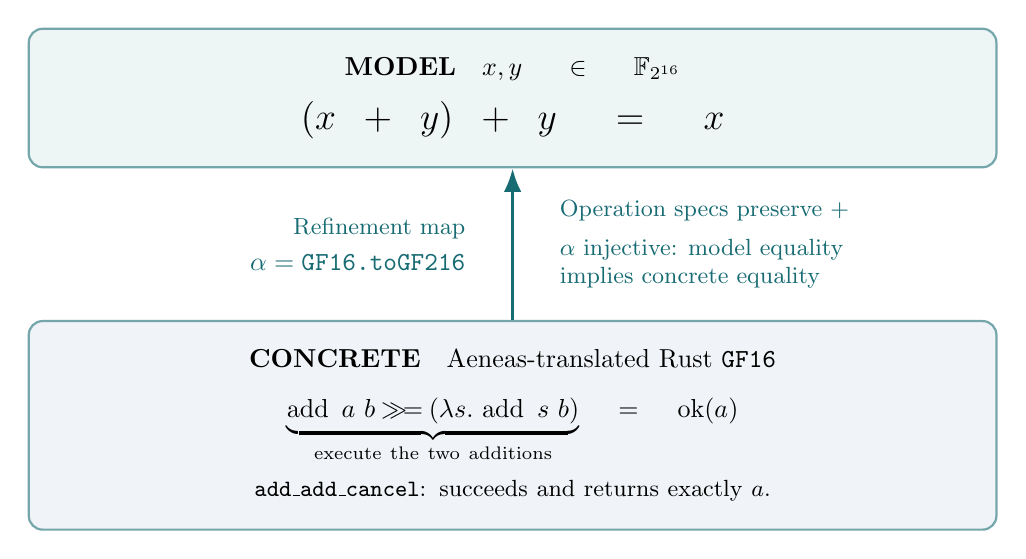
\begin{tikzpicture}[scale=0.94,transform shape]
\node[property,fill=modelbg] (model) {
  \textbf{MODEL}\quad $x,y\in\mathbb F_{2^{16}}$\\[7pt]
  {\Large $(x+y)+y=x$}
};
\node[property,fill=concretebg,below=2.05cm of model] (concrete) {
  \textbf{CONCRETE}\quad Aeneas-translated Rust \texttt{GF16}\\[7pt]
  $\underbrace{\cadd\ a\ b\bind(\lambda s.\,\cadd\ s\ b)}_{\text{execute the two additions}}=\ok(a)$\\[6pt]
  {\small \texttt{add\_add\_cancel}: succeeds and returns exactly $a$.}
};
\draw[refinement] (concrete.north) -- (model.south)
  node[midway,left=5mm,align=right] {\small Refinement map\\[2pt]
    $\alpha=\texttt{GF16.toGF216}$}
  node[midway,right=5mm,align=left] {\small Operation specs preserve $+$\\[3pt]
    \small $\alpha$ injective: model equality\\[-1pt]
    \small implies concrete equality};
\end{tikzpicture}

\smallskip
{\small $\ok(r)$ means \textbf{successful execution returning the value $r$}.}
\end{frame}

\begin{frame}{Distributivity}
\centering
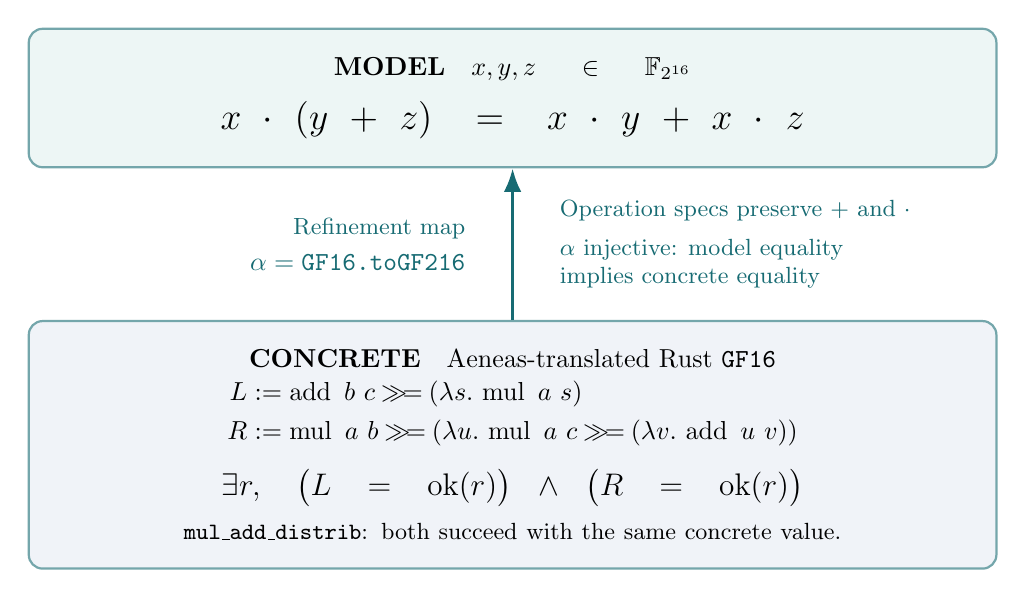
\begin{tikzpicture}[scale=0.94,transform shape]
\node[property,fill=modelbg] (model) {
  \textbf{MODEL}\quad $x,y,z\in\mathbb F_{2^{16}}$\\[7pt]
  {\Large $x\cdot(y+z)=x\cdot y+x\cdot z$}
};
\node[property,fill=concretebg,below=2.05cm of model] (concrete) {
  \textbf{CONCRETE}\quad Aeneas-translated Rust \texttt{GF16}\\[3pt]
  $\begin{aligned}
    L&:=\cadd\ b\ c\bind(\lambda s.\,\cmul\ a\ s)\\
    R&:=\cmul\ a\ b\bind(\lambda u.\,\cmul\ a\ c\bind(\lambda v.\,\cadd\ u\ v))
  \end{aligned}$\\[7pt]
  {\large $\exists r,\quad \bigl(L=\ok(r)\bigr)\ \land\ \bigl(R=\ok(r)\bigr)$}\\[5pt]
  {\small \texttt{mul\_add\_distrib}: both succeed with the same concrete value.}
};
\draw[refinement] (concrete.north) -- (model.south)
  node[midway,left=5mm,align=right] {\small Refinement map\\[2pt]
    $\alpha=\texttt{GF16.toGF216}$}
  node[midway,right=5mm,align=left] {\small Operation specs preserve $+$ and $\cdot$\\[3pt]
    \small $\alpha$ injective: model equality\\[-1pt]
    \small implies concrete equality};
\end{tikzpicture}

\smallskip
{\small $\ok(r)$ means \textbf{successful execution returning the value $r$}.}
\end{frame}


\begin{frame}{Five key statements behind the examples}
\centering
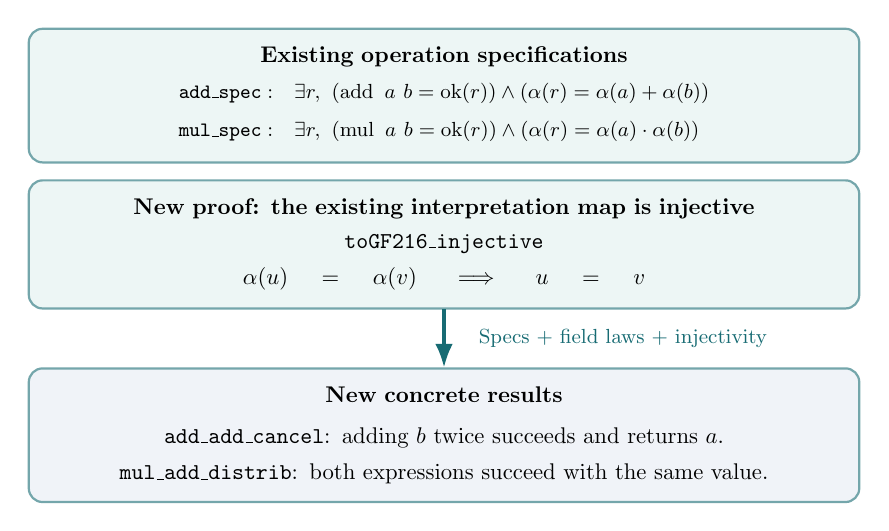
\begin{tikzpicture}[scale=0.82,transform shape]
\node[property,fill=modelbg,inner sep=8pt] (specs) {
  \textbf{Existing operation specifications}\\[5pt]
  \small
  $\begin{aligned}
  \texttt{add\_spec}:\quad&\exists r,\ (\cadd\ a\ b=\ok(r))\land
     (\alpha(r)=\alpha(a)+\alpha(b))\\[3pt]
  \texttt{mul\_spec}:\quad&\exists r,\ (\cmul\ a\ b=\ok(r))\land
     (\alpha(r)=\alpha(a)\cdot\alpha(b))
  \end{aligned}$
};
\node[property,fill=modelbg,inner sep=8pt,below=0.25cm of specs] (bridge) {
  \textbf{New proof: the existing interpretation map is injective}\\[3pt]
  \texttt{toGF216\_injective}\\[4pt]
  $\alpha(u)=\alpha(v)\ \Longrightarrow\ u=v$
};
\node[property,fill=concretebg,inner sep=8pt,below=0.9cm of bridge] (results) {
  \textbf{New concrete results}\\[6pt]
  \texttt{add\_add\_cancel}: adding $b$ twice succeeds and returns $a$.\\[4pt]
  \texttt{mul\_add\_distrib}: both expressions succeed with the same value.
};
\draw[refinement] (bridge.south) -- (results.north)
  node[midway,right=4mm] {\small Specs + field laws + injectivity};
\end{tikzpicture}

\smallskip
{\scriptsize $\ok(r)$ means \textbf{successful execution returning the value $r$}.\\[2pt]
$\alpha=\texttt{GF16.toGF216}$. Cancellation uses \texttt{add\_spec} and injectivity;
 distributivity also uses \texttt{mul\_spec}.\\
These are the presentation's key statements; underlying arithmetic and execution lemmas are omitted.}
\end{frame}

% Sources:
% Spqr/Math/Gf16/Field.lean: GF16.toGF216 and toGF216_injective.
% Spqr/Specs/Encoding/Gf/GF16/Add.lean: add_spec, add_add_cancel.
% Spqr/Specs/Encoding/Gf/GF16/Mul.lean: mul_spec, mul_add_distrib.
% Bind notation: m >>= (lambda x. n) runs m and passes its successful result to n.
% The upward arrow is the concrete-to-model interpretation, not its inverse.
% Operation specifications guarantee successful execution and preserve field operations;
% injectivity reflects the resulting model equality back to concrete GF16 values.
\end{document}
